%!TeX root=../tese.tex
%(dica para o editor de texto: este arquivo é parte de um documento maior)
% para saber mais: https://tex.stackexchange.com/q/78101/183146

\chapter{Procedimentos de comparação e resultados}
\label{cap:comparacao}

Neste capítulo serão definidos procedimentos de modelagem alternativos às séries temporais financeiras de taxas de câmbio. Um dos modelos é o modelo paramétrico \eng{ARIMA}, estudado no Capítulo \ref{cap:series}. 

O outro será um modelo não-paramétrico criado com redes neurais, estudadas no Capítulo \ref{cap:perceptron}, sendo utilizadas redes neurais recorrentes, devido à sua arquitetura mais condizente com o problema em questão, de acordo com Kopec \citep{classic} e Géron \citep{hands}.

A seguir, serão feitas comparações entre os modelos preditivos de séries temporais, através de medidas de desempenho comuns como as funções de erros RMSE\footnote{Raiz do erro quadrático médio} e MAE\footnote{Erro absoluto médio} e o coeficiente de correlação de \eng{Pearson}  entre os valores previstos e conhecidos do conjunto de teste.

\section{Modelagem e procedimentos gerais}

A princípio, foi escolhido um período com os valores em Reais de cotações de venda do Dólar. Esse período de dados foi dividido em \emph{janelas de dados} móveis e de tamanho fixo. Considere o seguinte exemplo. 

Seja a sequência de números de $0$ a $9$: $(0,1,2,3,4,5,6,7,8,9)$. Suponha que queremos criar janelas de dados de tamanho $6$, elas seriam uma sequência de sequências:
\[ ((0,1,2,3,4,5),(1,2,3,4,5,6),(2,3,4,5,6,7),(3,4,5,6,7,8),(4,5,6,7,8,9)) \]

Perceba que criamos, a partir da sequência de $10$ números original, $5$ janelas com $6$ números cada, o tamanho de cada uma. Generalizando, se temos $N$ dados, podemos criar $N{-}M{+}1$ janelas de dados de tamanho $M$.

A ideia geral é usar essas janelas de dados para treinar modelos que descrevam a série de cotações. Numa série temporal financeira, temos os valores passados, e podemos querer prever valores futuros apenas com as informações que temos do passado.

Os dados de cotação de venda do Dólar utilizados nesse trabalho foram obtidos via download de arquivo CSV disponível no site do Banco Central do Brasil\footnote{\url{https://olinda.bcb.gov.br/olinda/servico/PTAX/versao/v1/aplicacao}}, sendo que optei por baixar dados de cotações desde o ano de $2010$ até a data atual em que isso foi feito, para depois pudesse escolher os períodos que julgasse necessário.

\section{Primeiro teste: Prevendo 7 dias}

Neste primeiro teste filtrei os dados para um período específico, que vai de Julho/2016 até Dezembro/2017, ou seja, totalizando $18$ meses de dados. Essa série temporal é mostrada na Figura \ref{fig:serie_1}, abaixo.

\begin{figure}[htb]
\centering
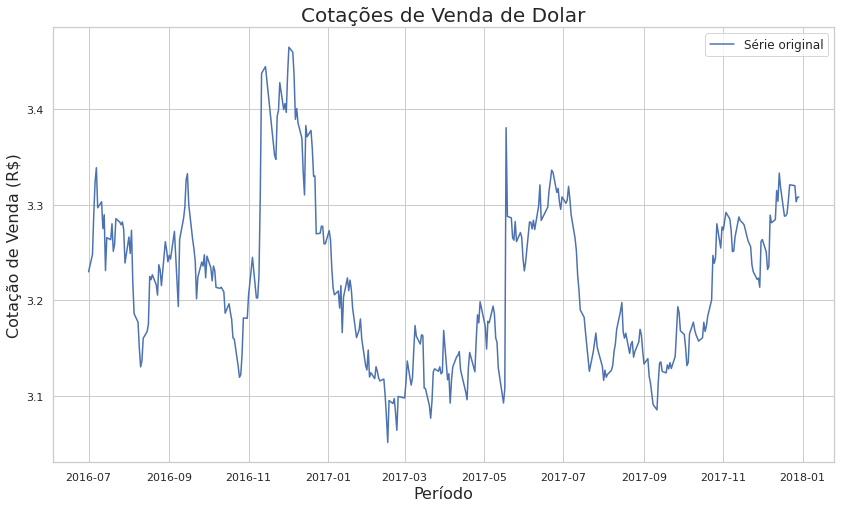
\includegraphics[width=14cm]{figuras/serie_1}
\caption{Cotações de venda do Dólar em Reais. Período: Jul/2016 - Dez/2017.}
\label{fig:serie_1}
\end{figure}

De forma a treinar os modelos de forma mais justa, foi definido que serão utilizadas janelas de $30$ dias de valores de câmbios passados para prever o valor de câmbio do dia imediatamente a seguir. Por exemplo, suponha que tenhamos uma janela com valores dos $30$ dias de Junho, essa janela será uma série temporal que será modelada e então cada modelo irá prever a taxa de câmbio do dia $1$° de Julho.

Isto não está exato, pois a série não possui dados para cada dia do ano, apenas para dias úteis, pulando finais de semana e feriados. Na prática, escolhi para esse primeiro teste, prever os valores da série no período que vai de $16/08/2017$ até $24/08/2017$. 

Dessa forma, utilizando as janelas de $30$ dias passados, de acordo com os dias úteis disponíveis, criei as $7$ janelas, sendo que a primeira tem seus $30$ valores contidos no período de $05/07/2017$ a $15/08/2017$, e assim sucessivamente para as próximas janelas.

Realizei os procedimentos de treinamento, tanto para o modelo ARIMA, quanto para os modelos de redes neurais. Um deles utilizando o \eng{Keras} e outro utilizando a implementação própria do \eng{Perceptron}. Adicionalmente, foram incluídos dois simples modelos de referência, a partir da média móvel, uma com $7$ dias e a outra com $30$ dias, como sendo a previsão para o próximo dia. 

Cada modelo possui suas particularidades na fase de treinamento. Para listá-las e deixar claro as diferenças entre os modelos ARIMA e do Keras, foi construída a Tabela \ref{tabela:params_0}.

\begin{table}[]
\begin{center}
\resizebox{\textwidth}{!}{
\begin{tabular}{|p{0.24\linewidth}|p{0.32\linewidth}|p{0.32\linewidth}|}
\hline
\textbf{Modelo} & \textbf{ARIMA} & \textbf{Modelo Neural} \\
\hline
\hline
\multirow{2}{*}{\textbf{Treino do modelo}} 
& - Nenhuma janela anterior (Apenas os $30$ dias de cada janela); & - $253$ janelas anteriores de $30$ dias cada e mais o próximo dia conhecido;  \\
& - Calibração automática dos parâmetros (autocorrelação). & - Calibração manual dos parâmetros. \\
\hline
\textbf{Teste do modelo} 
& - $7$ dias futuros ($1$ dia de cada uma das janelas de treino). & - $7$ janelas de $30$ dias cada. \\
\hline
\end{tabular}}
\caption{Especificação dos dados de treino e de teste ($7$ dias).}\label{tabela:params_0}
\end{center}
\end{table}

Tais previsões foram realizadas por modelos que foram treinados após a configuração dos hiperparâmetros de cada modelo. No caso do ARIMA é possível identificá-los utilizando a função de autocorrelação, já nos modelos de redes neurais é feito por tentativa-e-erro com algum conhecimento prévio do tipo de dado usado, nesse caso, financeiros, o que já determina para o Keras o modelo de redes recorrentes, por exemplo. 

Para todos os modelos também seria possível realizar uma busca exaustiva de parâmetros (\eng{grid search}) de forma que o melhor conjunto de parâmetros é escolhido a partir de alguma métrica do treinamento, isto é, o conjunto que se sai melhor nessa métrica. 

Esse procedimento foi realizado para o modelo ARIMA, e ele identificou os mesmos parâmetros que as funções de autocorrelação identificaram, e eles foram os mesmos para as $7$ janelas de teste, e estão listados na Tabela \ref{tabela:params_1}.

\begin{table}[]
\begin{center}
\begin{tabular}{|ll|c|}
\hline
\multicolumn{2}{|c|}{\textbf{Hiperparâmetros do}} & \multirow{2}{*}{\textbf{Valor}} \\
\multicolumn{2}{|c|}{\textbf{Modelo ARIMA}} & \\
\hline
\hline
\eng{p} & Componente autoregressiva & $2$ \\
\eng{d} & Componente de diferenças & $0$ \\
\eng{q} & Componente de média-móvel & $0$ \\
\hline
\end{tabular}
\caption{Hiperparâmetros do modelo ARIMA ($7$ dias).}\label{tabela:params_1}
\end{center}
\end{table}

Por sua vez, os hiperparâmetros das redes neurais Keras estão listados na Tabela \ref{tabela:params_2}, e da rede Perceptron implementada, estão listados na Tabela \ref{tabela:params_3}.

\begin{table}[]
\begin{center}
\begin{tabular}{|ll|c|}
\hline
\multicolumn{2}{|c|}{\textbf{Hiperparâmetros do}} & \multirow{2}{*}{\textbf{Valor}} \\
\multicolumn{2}{|c|}{\textbf{Modelo Neural (Keras)}} & \\
\hline
\hline
\eng{filters} & Qtde de filtros & $64$ \\
\eng{kernel$\_$size} & Qtde de neurônios por filtro & $3$ \\
\eng{activation} & Função de ativação & `elu' \\
\eng{padding} & Ordem dos dados & `causal' \\
\eng{input$\_$shape} & Formato de entrada e saída & $(30, 1)$ \\
\eng{pool$\_$size} & Unidades de votação & $3$ \\
\eng{optimizer} & Método de otimização & `adam' \\
\eng{loss} & Função de perda & `mse' \\
\eng{epochs} & Épocas de treinamento & $15$ \\
\hline
\end{tabular}
\caption{Hiperparâmetros do modelo neural Keras.}\label{tabela:params_2}
\end{center}
\end{table}


\begin{table}[]
\begin{center}
\begin{tabular}{|ll|c|}
\hline
\multicolumn{2}{|c|}{\textbf{Hiperparâmetros do}} & \multirow{2}{*}{\textbf{Valor}} \\
\multicolumn{2}{|c|}{\textbf{Modelo Neural (Perceptron)}} & \\
\hline
\hline
\eng{taxa} & Taxa de aprendizado & $0.001$ \\
\eng{ativacao} & Função de ativação & `elu' \\
\eng{N} & Arquitetura da rede & $[20, 10, 1]$ \\
\eng{M} & Épocas de treinamento & $25$ \\
\hline
\end{tabular}
\caption{Hiperparâmetros do modelo neural Perceptron.}\label{tabela:params_3}
\end{center}
\end{table}

Ao final dos treinamentos e previsões, listei na Tabela \ref{tabela:teste_7} os resultados de cada modelo, e nas últimas linhas as métricas de avaliação já definidas acima.

\begin{table}[]
\begin{center}
\resizebox{\textwidth}{!}{
\begin{tabular}{|c|c|c|c|c|c|c|}
\hline
\multirow{2}{*}{\textbf{Dia}} & \multirow{2}{*}{\textbf{Cotação}} 
& \textbf{Média-Móvel} & \textbf{Média-Móvel}
& \multirow{2}{*}{\textbf{ARIMA}} 
& \textbf{Rede Neural} & \textbf{Rede Neural} \\
&& \textbf{(7 dias)} & \textbf{(30 dias)}
&& \textbf{(Keras)} & \textbf{(Perceptron)} \\
\hline
\hline
16/08/2017 & 3.167 & 3.305 & 3.177 & 3.204 & 3.177 & 3.198 \\
17/08/2017 & 3.160 & 3.304 & 3.172 & 3.151 & 3.174 & 3.465 \\
18/08/2017 & 3.165 & 3.306 & 3.167 & 3.158 & 3.169 & 3.172 \\
21/08/2017 & 3.144 & 3.304 & 3.163 & 3.169 & 3.163 & 3.154 \\
22/08/2017 & 3.154 & 3.302 & 3.159 & 3.137 & 3.159 & 3.223 \\
23/08/2017 & 3.157 & 3.305 & 3.156 & 3.159 & 3.156 & 3.154 \\
24/08/2017 & 3.140 & 3.308 & 3.154 & 3.158 & 3.153 & 3.154 \\
\hline
\hline
\textbf{MAE} & - & 0.150 & 0.009 & 0.016 & 0.009 & 0.063 \\
\textbf{RMSE} & - & 0.150 & 0.011 & 0.020 & 0.011 & 0.119 \\
\textbf{Pearson} & - & -0.202 & 0.737 & 0.320 & 0.759 & 0.305 \\
\hline
\end{tabular}}
\caption{Previsões para $7$ dias e métricas dos modelos das janelas de cotações do Dólar.}\label{tabela:teste_7}
\end{center}
\end{table}

A seguir, na Figura \ref{fig:series_previsoes_7_1}, estão os gráficos dos modelos desses $7$ dias de previsão para os modelos que se saíram melhores, ou seja, Rede Neural Keras, Média-Móvel $30$ dias e ARIMA.

\begin{figure}[htb]
\centering
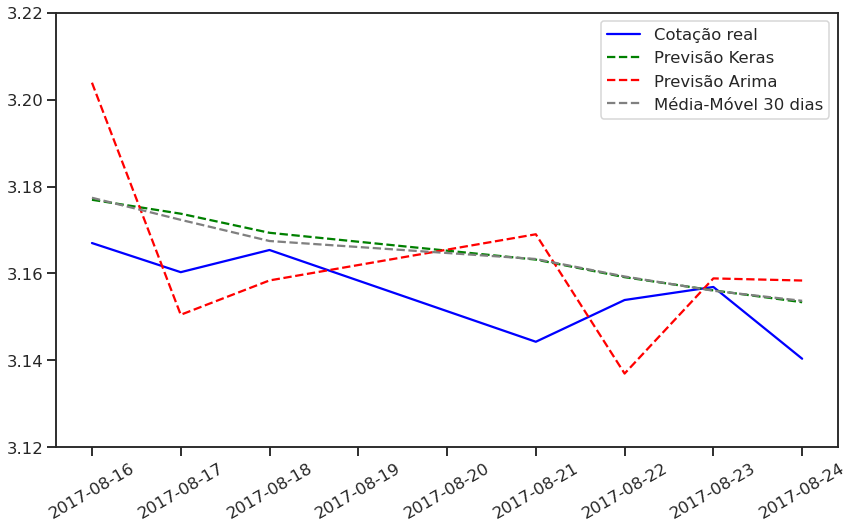
\includegraphics[width=14cm]{figuras/series_previsoes_7_1}
\caption{Previsões de $7$ dias dos modelos ARIMA, Rede Neural Keras e Média-Móvel $30$ dias das janelas de cotações do Dólar.}
\label{fig:series_previsoes_7_1}
\end{figure}

Já na Figura \ref{fig:series_previsoes_7_2} estão os gráficos dos modelos que não tiveram um bom desempenho, o Média-Móvel $7$ dias e o Rede Neural Perceptron.

\begin{figure}[htb]
\centering
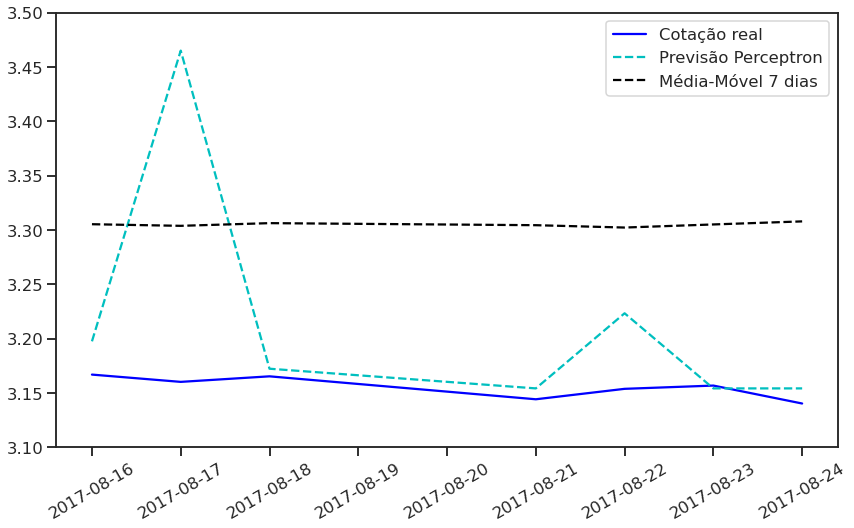
\includegraphics[width=14cm]{figuras/series_previsoes_7_2}
\caption{Previsões de $7$ dias do modelo de rede Perceptron e de Média-Móvel de $7$ dias das janelas de cotações do Dólar.}
\label{fig:series_previsoes_7_2}
\end{figure}

A partir dos resultados vimos que, para estas $7$ janelas de treino, o modelo Keras foi o que se saiu melhor, enquanto que o modelo Perceptron se saiu bem pior do que ele, o que era de certa forma esperado, já que utiliza uma arquitetura não otimizada para o problema em questão, o que já serviu de verificação deste fato.

O ARIMA saiu-se melhor que o Perceptron, mas nem tão bom quanto o modelo neural recorrente do Keras. O modelo neural não utilizou pressupostos sobre os dados, apenas uma grande quantidade de dados de treinamento, o que é requisito para seu funcionamento e utilização.

Apesar disso, o modelo de referência, a Média-Móvel $30$ dias de cada janela, saiu-se tão bem quanto o modelo neural Keras. Indicação que o modelo poderia se sair ainda melhor, se tivesse sido fornecido a ele ainda mais dados, uma vez que ele é de fato um modelo de aprendizagem profunda, funcionando tão bem quanto mais dados há disponíveis.

Já o modelo de Média-Móvel $7$ dias foi o pior dentre todos os modelos, com seus valores previstos estando em outro patamar, sendo inclusive pior em média do que o Perceptron.

Não há como treinar um modelo de redes neurais sem uma quantidade razoável de exemplos, nesse caso, de janelas de dados do passado. Na verdade, como foram utilizadas janelas correspondentes a quase um ano de dados do passado, o percentual entre dados de teste $/$ dados de treino foi pouco menor de $3\%$, ou seja, a eficiência do modelo, apesar de impressionante, era de certa forma esperada.

O modelo ARIMA é paramétrico, e de natureza estatística, dessa forma ele gera previsões que são estimativas contidas dentro de um intervalo de confiança. Tal intervalo foi calculado, com nível de $95\%$ de confiança, e pode ser visto na Figura \ref{fig:series_previsoes_7_3}.

\begin{figure}[htb]
\centering
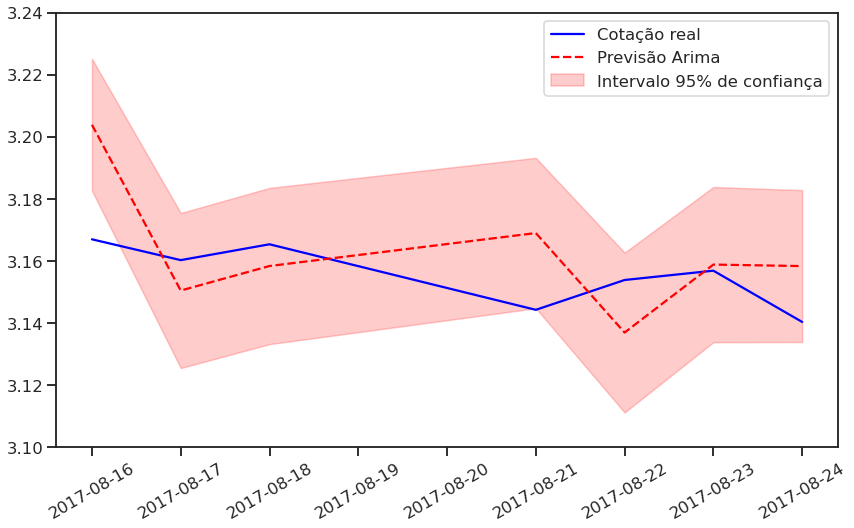
\includegraphics[width=14cm]{figuras/series_previsoes_7_3}
\caption{Previsões de $7$ dias do modelo ARIMA com o intervalo de $95\%$ de confiança para cada previsão.}
\label{fig:series_previsoes_7_3}
\end{figure}


\section{Segundo teste: Prevendo 30 dias}

Para investigar mais a fundo as relações entre tamanho do treino e do teste na avaliação dos modelos, um segundo teste foi realizado, agora com previsões para os próximos $30$ dias úteis, também começando a partir do dia $16/08/2017$, indo até o dia $27/09/2017$. 

Nesse teste é utilizada a mesma quantidade de dados de treinamento para os modelos neurais. Dessa vez, como estamos prevendo $30$ dias no futuro, com a mesma quantidade de dias do passado para o treino, a proporção entre dados de teste $/$ dados de treino subiu para aproximadamente $11\%$. Com isso, é esperado que a eficiência das redes neurais seja pior do que no teste anterior.

A tabela de especificação dos dados de treino e teste é também similar à do teste anterior, com algumas diferenças. Pode ser vista na Tabela \ref{tabela:params_5}.

\begin{table}[]
\begin{center}
\resizebox{\textwidth}{!}{
\begin{tabular}{|p{0.24\linewidth}|p{0.32\linewidth}|p{0.32\linewidth}|}
\hline
\textbf{Modelo} & \textbf{ARIMA} & \textbf{Modelo Neural} \\
\hline
\hline
\multirow{2}{*}{\textbf{Treino do modelo}} 
& - Nenhuma janela anterior (Apenas os $30$ dias de cada janela); & - $253$ janelas anteriores de $30$ dias cada e mais o próximo dia conhecido;  \\
& - Calibração automática dos parâmetros (\eng{grid search}). & - Calibração manual dos parâmetros. \\
\hline
\textbf{Teste do modelo} 
& - $30$ dias futuros ($1$ dia de cada uma das janelas de treino). & - $30$ janelas de $30$ dias cada. \\
\hline
\end{tabular}}
\caption{Especificação dos dados de treino e de teste ($30$ dias).}\label{tabela:params_5}
\end{center}
\end{table}

Sendo o mesmo conjunto de treino, não há necessidade novo treinamento das redes neurais, assim os hiperparâmetros são ainda os mesmos dados pelas Tabelas \ref{tabela:params_2} e \ref{tabela:params_3}. A diferença será no modelo ARIMA, já que cada janela de previsão é ajustada separadamente.

Dessa vez, a melhor estratégia foi utilizar o \eng{grid search}, que conforme descrito anteriormente, busca os melhores parâmetros de acordo com uma métrica do modelo \eng{ARIMA}. Esta métrica é a \defi{AIC} (\eng{Akaike Information Criterion}), que mede o quão bem um modelo ajusta-se aos dados sem gerar \eng{overfitting}.

Esta definição é utilizada por Sachin Date \citep{aic}, que complementa dizendo que esta métrica não faz tanto sentido se analisada sozinha, mas é melhor utilizada na comparação entre modelos, de forma que o modelo (os parâmetros utilizados, em nosso modelo ARIMA) com o menor valor de \eng{AIC} é o que terá o melhor balanço entre ajuste aos dados de treino e menor \eng{overfitting} durante as previsões.

Já que a alternativa seria analisar $30$ gráficos de autocorrelação e outros $30$ gráficos de autocorrelação parcial, e a busca irá tentar otimizar os parâmetros com a métrica que minimiza o \eng{overfitting}, não há desvantagens nessa estratégia, e os parâmetros ótimos encontrados de cada janela foram utilizados nas previsões.

Como há um número grande de parâmetros ótimos, $30$ de cada um dos $3$ parâmetros do modelo ARIMA, foram resumidos em \eng{boxplot's}, que podem ser visualizados na Figura \ref{fig:arima_boxplot_30}.

\begin{figure}[htb]
\centering
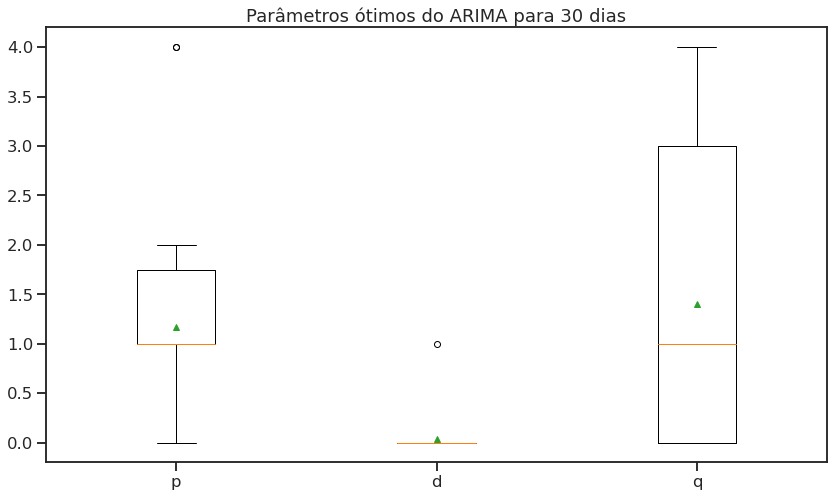
\includegraphics[width=11cm]{figuras/arima_boxplot_30}
\caption{Previsões para $30$ dias dos modelos ARIMA e Rede Neural (Keras) das janelas de cotações do Dólar.}
\label{fig:arima_boxplot_30}
\end{figure}

Estão listados na Tabela \ref{tabela:teste_30} os resultados de cada modelo, e nas últimas linhas as métricas de avaliação previamente definidas.

% \begin{table}[]
% \begin{center}
\footnotesize
\begin{longtable}{|c|c|c|c|c|c|c|}
\hline

\captionlistentry{Previsões para $30$ dias e métricas dos modelos das janelas de cotações do Dólar.}\label{tabela:teste_30}

\multirow{2}{*}{\textbf{Dia}} & \multirow{2}{*}{\textbf{Cotação}} 
& \textbf{Média-Móvel} & \textbf{Média-Móvel}
& \multirow{2}{*}{\textbf{ARIMA}} 
& \textbf{Rede Neural} & \textbf{Rede Neural} \\
&& \textbf{(7 dias)} & \textbf{(30 dias)}
&& \textbf{(Keras)} & \textbf{(Perceptron)} \\
\hline

\endhead

\hline
\multicolumn{7}{|r|}{\textit{continua}\enspace$\longrightarrow$}\\
\hline
\caption[]{Previsões para $30$ dias e métricas dos modelos das janelas de cotações do Dólar.}

\endfoot

\hline
\caption[]{Previsões para $30$ dias e métricas dos modelos das janelas de cotações do Dólar.}

\endlastfoot

\hline
16/08/2017 & 3.167 & 3.271 & 3.177 & 3.211 & 3.177 & 3.198 \\
17/08/2017 & 3.160 & 3.273 & 3.172 & 3.149 & 3.174 & 3.465 \\
18/08/2017 & 3.165 & 3.274 & 3.167 & 3.158 & 3.169 & 3.172 \\
21/08/2017 & 3.144 & 3.273 & 3.163 & 3.169 & 3.163 & 3.154 \\
22/08/2017 & 3.154 & 3.265 & 3.159 & 3.137 & 3.159 & 3.223 \\
23/08/2017 & 3.157 & 3.258 & 3.156 & 3.159 & 3.156 & 3.154 \\
24/08/2017 & 3.140 & 3.249 & 3.154 & 3.153 & 3.153 & 3.154 \\
25/08/2017 & 3.146 & 3.241 & 3.151 & 3.142 & 3.149 & 3.223 \\
28/08/2017 & 3.156 & 3.234 & 3.150 & 3.150 & 3.143 & 3.223 \\
29/08/2017 & 3.170 & 3.235 & 3.149 & 3.152 & 3.138 & 3.223 \\
30/08/2017 & 3.164 & 3.236 & 3.149 & 3.172 & 3.135 & 3.221 \\
31/08/2017 & 3.147 & 3.238 & 3.149 & 3.160 & 3.134 & 3.223 \\
01/09/2017 & 3.133 & 3.238 & 3.150 & 3.143 & 3.136 & 3.221 \\
04/09/2017 & 3.139 & 3.240 & 3.150 & 3.120 & 3.140 & 3.221 \\
05/09/2017 & 3.120 & 3.249 & 3.150 & 3.150 & 3.143 & 3.221 \\
06/09/2017 & 3.113 & 3.259 & 3.149 & 3.120 & 3.142 & 3.221 \\
08/09/2017 & 3.091 & 3.262 & 3.147 & 3.125 & 3.142 & 3.221 \\
11/09/2017 & 3.085 & 3.270 & 3.145 & 3.097 & 3.142 & 3.221 \\
12/09/2017 & 3.114 & 3.277 & 3.143 & 3.090 & 3.139 & 3.223 \\
13/09/2017 & 3.134 & 3.292 & 3.142 & 3.128 & 3.138 & 3.223 \\
14/09/2017 & 3.135 & 3.304 & 3.143 & 3.143 & 3.137 & 3.223 \\
15/09/2017 & 3.126 & 3.303 & 3.143 & 3.136 & 3.137 & 3.223 \\
18/09/2017 & 3.124 & 3.304 & 3.143 & 3.125 & 3.136 & 3.223 \\
19/09/2017 & 3.132 & 3.305 & 3.143 & 3.128 & 3.135 & 3.223 \\
20/09/2017 & 3.128 & 3.304 & 3.144 & 3.137 & 3.135 & 3.297 \\
21/09/2017 & 3.135 & 3.306 & 3.143 & 3.128 & 3.134 & 3.170 \\
22/09/2017 & 3.128 & 3.304 & 3.143 & 3.140 & 3.138 & 3.170 \\
25/09/2017 & 3.141 & 3.302 & 3.142 & 3.128 & 3.144 & 3.154 \\
26/09/2017 & 3.167 & 3.305 & 3.141 & 3.142 & 3.144 & 3.172 \\
27/09/2017 & 3.193 & 3.308 & 3.141 & 3.171 & 3.142 & 3.223 \\
\hline
\hline
\textbf{MAE} & - & 0.132 & 0.018 & 0.014 & 0.016 & 0.076 \\
\textbf{RMSE} & - & 0.137 & 0.023 & 0.017 & 0.022 & 0.097 \\
\textbf{Pearson} & - & -0.075 & 0.366 & 0.723 & 0.383 & 0.008 \\

\end{longtable}
% \end{center}
% \end{table}
\normalsize

A seguir, na Figura \ref{fig:series_previsoes_30_1}, estão os gráficos dos modelos dos $30$ dias de previsão, os quais se sairam melhores de acordo com as métricas na tabela acima. Na Figura \ref{fig:series_previsoes_30_2}, estão os gráficos dos demais modelos utilizados para previsão, que não tiveram desempenho tão bom quanto os anteriores.

\begin{figure}[htb]
\centering
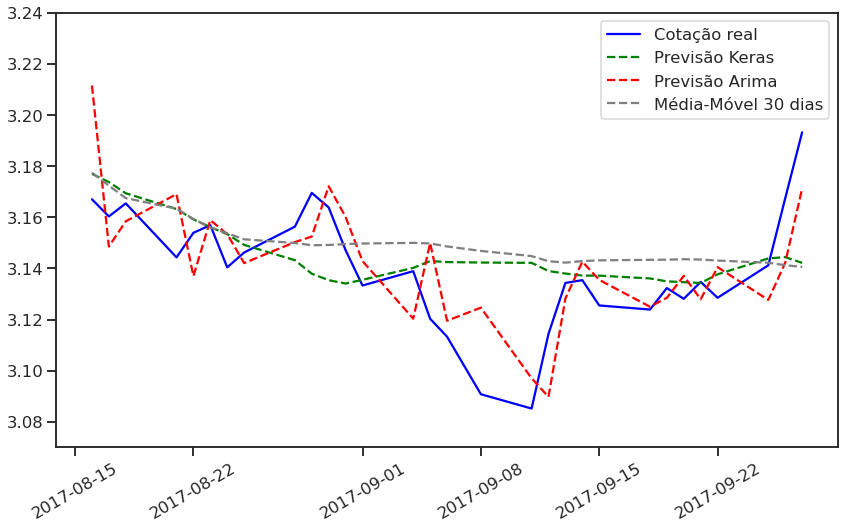
\includegraphics[width=14cm]{figuras/series_previsoes_30_1}
\caption{Previsões de $30$ dias dos modelos ARIMA, Rede Neural Keras e Média-Móvel $30$ dias das janelas de cotações do Dólar.}
\label{fig:series_previsoes_30_1}
\end{figure}

\begin{figure}[htb]
\centering
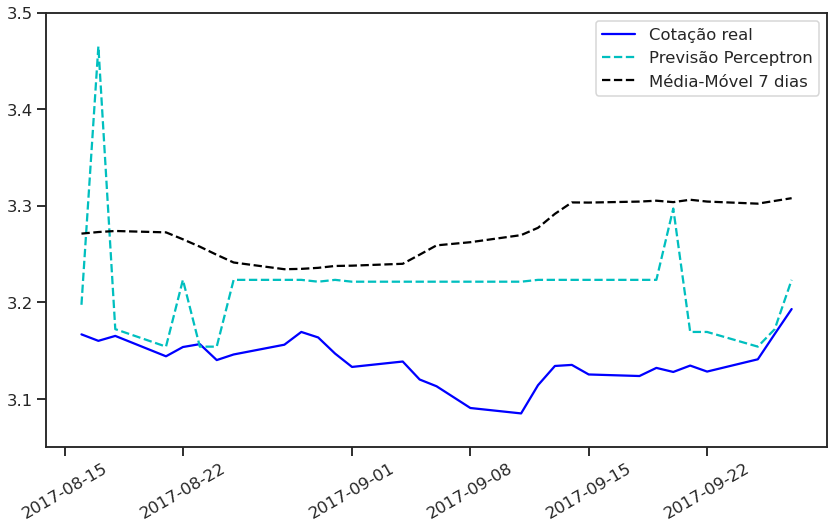
\includegraphics[width=14cm]{figuras/series_previsoes_30_2}
\caption{Previsões de $30$ dias do modelo de rede Perceptron e de Média-Móvel de $7$ dias das janelas de cotações do Dólar.}
\label{fig:series_previsoes_30_2}
\end{figure}

Novamente é exibido, na Figura \ref{fig:series_previsoes_30_3}, o gráfico com o intervalo de $95\%$ de confiança para cada uma das $30$ previsões do modelo ARIMA.

\begin{figure}[htb]
\centering
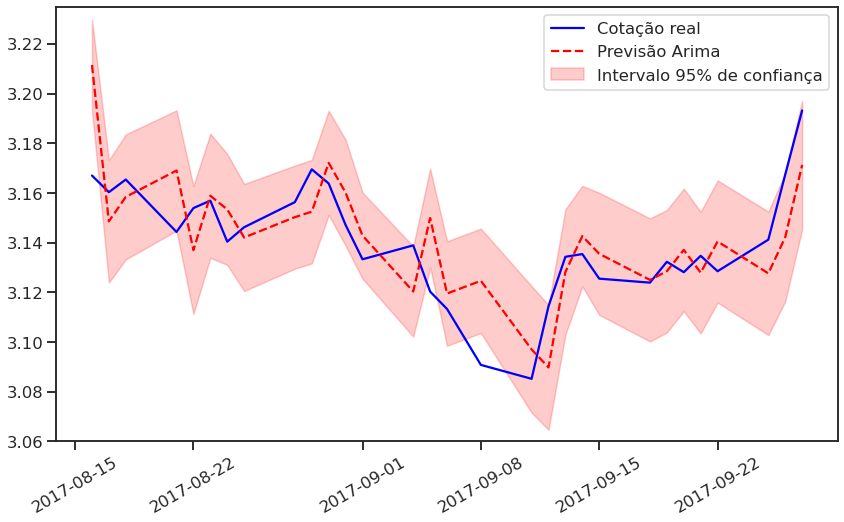
\includegraphics[width=14cm]{figuras/series_previsoes_30_3}
\caption{Previsões de $30$ dias do modelo ARIMA com o intervalo de $95\%$ de confiança para cada previsão.}
\label{fig:series_previsoes_30_3}
\end{figure}

Nota-se que a previsão de $30$ dias no futuro, partindo do mesmo ponto que no teste anterior, colocou o modelo \eng{ARIMA} em primeiro lugar, sendo que em segundo ficou a rede neural Keras praticamente empatado com a Média-Móvel $30$ dias.

Se observarmos na Figura \ref{fig:series_previsoes_30_1}, há um vale nos valores de cotação próximo ao dia $08/09/2017$, e apenas as previsões do \eng{ARIMA} acompanham esse vale, o que faz com que seus resultados médios sejam superiores aos demais modelos, nesse caso. Os demais modelos tiveram os mesmos resultados, na mesma ordenação que no teste anterior.

\section{Terceiro teste: Prevendo 1 ano}

Para este teste, um período maior de tempo foi utilizado, de forma a poder fornecer uma quantidade razoável de exemplos para o treino das redes neurais. O período de cotações do Dólar utilizado pode ser visto na Figura \ref{fig:keras_treino_ano}, e totaliza $3$ anos e meio, de forma que $75\%$ deste período é o conjunto de treino e o restante, totalizando $1$ ano, será o período de teste de todos os modelos.

\begin{figure}[htb]
\centering
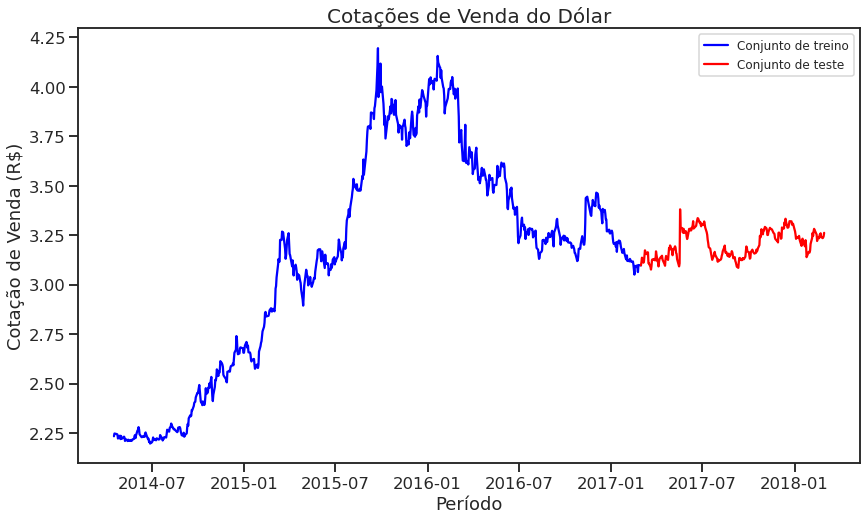
\includegraphics[width=14cm]{figuras/keras_treino_ano}
\caption{Período da série temporal das cotações do Dólar, especificando os conjuntos de treino (em azul) das redes neurais e o conjunto de teste (em vermelho) de todos os modelos.}
\label{fig:keras_treino_ano}
\end{figure}

O total de dias úteis que serão previstos e comparados com a curva vermelha no gráfico da Figura \ref{fig:keras_treino_ano} é $250$. Foram feitos novos treinamentos e procedimento para escolha dos melhores parâmetros de cada modelo.

A tabela de especificação dos dados de treino e teste foi feita nos moldes dos testes anteriores, com algumas diferenças importantes, e pode ser vista na Tabela \ref{tabela:params_ano_1}.

\begin{table}[]
\begin{center}
\begin{tabular}{|p{0.24\linewidth}|p{0.32\linewidth}|p{0.32\linewidth}|}
\hline
\textbf{Modelo} & \textbf{ARIMA} & \textbf{Modelo Neural} \\
\hline
\hline
\multirow{2}{*}{\textbf{Treino do modelo}} 
& - Nenhuma janela anterior (Apenas os $30$ dias de cada janela); & - $722$ janelas anteriores de $30$ dias cada e mais o próximo dia conhecido;  \\
& - Calibração automática dos parâmetros (\eng{grid search}). & - Calibração manual dos parâmetros. \\
\hline
\textbf{Teste do modelo} 
& - $250$ dias futuros ($1$ dia de cada uma das janelas de treino). & - $250$ janelas de $30$ dias cada. \\
\hline
\end{tabular}
\caption{Especificação dos dados de treino e de teste ($1$ ano).}\label{tabela:params_ano_1}
\end{center}
\end{table}

Dessa vez, para o ARIMA, também foi realizado o procedimento de \eng{grid search}, e para se fazer um chute de qual ordem máxima de cada componente que seria utilizada na busca, apliquei as funções de autocorrelação e de autocorrelação parcial em cada uma das $250$ janelas de previsão. 

De forma a exibir de forma resumida os resultados, desenhei um \eng{boxplot} para cada uma das funções, que irá mostrar a distribuição dos \eng{lags} significativos \footnote{Cujo valor não está no intervalo de confiança que representa autocorrelação nula naquele \eng{lag}.} máximos que elas retornaram para as janelas, que podem ser vistos na Figura \ref{fig:arima_acf}.

\begin{figure}[htb]
\centering
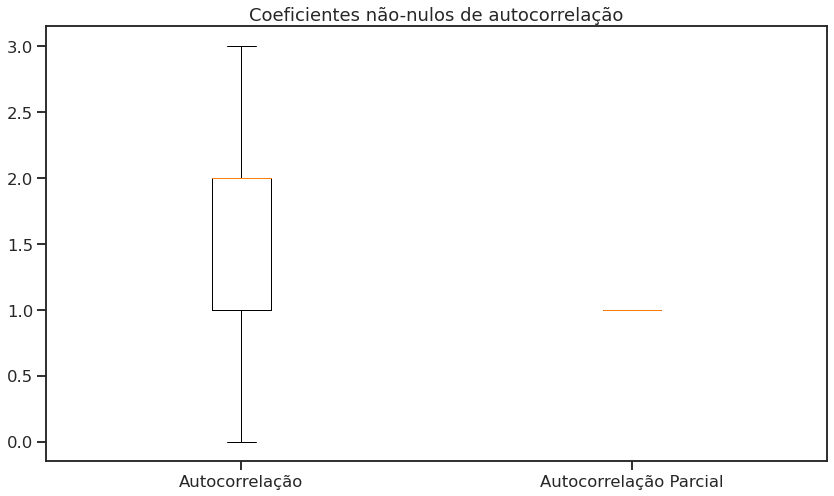
\includegraphics[width=11cm]{figuras/arima_acf}
\caption{Distribuição dos \eng{lags} significativos máximos para as funções de autocorrelação (esquerda) e de autocorrelação parcial (direita).}
\label{fig:arima_acf}
\end{figure}

Pela Figura \ref{fig:arima_acf}, analisando o \eng{boxplot} da esquerda, podemos notar que em média um componente de autocorrelação $p$ ideal estaria entre $1$ e $3$, com mais probabilidade nos valores menores, enquanto isso a função de autocorrelação parcial, na direita, não foi muito informativo, sendo basicamente constante igual a $1$ para todas as janelas.

Realizando o \eng{grid search}, o modelo otimizou sua métrica em cada janela, fornecendo a melhor escolha dos parâmetros $(p, d, q)$, de acordo com sua métrica usual que envolve minimização de entropia, e de forma a resumir a escolha para as $250$ janelas, foram construídos $3$ \eng{boxplot's}, um para cada parâmetro, que podem ser vistos na Figura \ref{fig:arima_boxplot}.

\begin{figure}[htb]
\centering
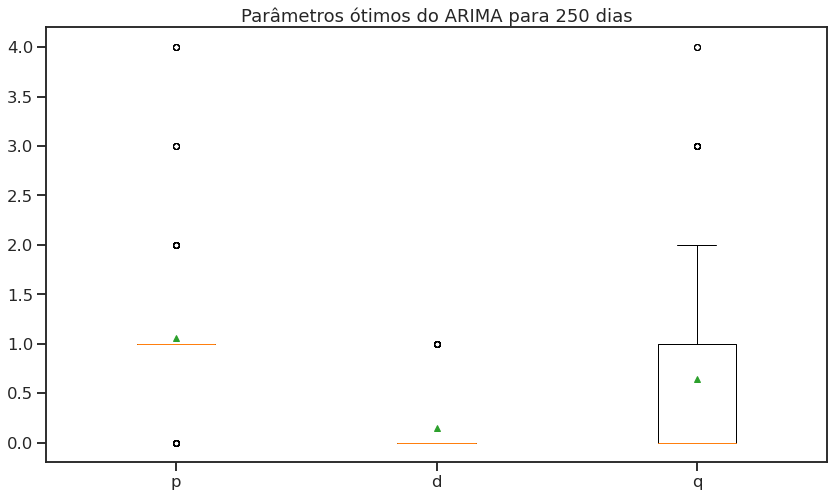
\includegraphics[width=11cm]{figuras/arima_boxplot}
\caption{Distribuição dos parâmetros ótimos $(p, q, d)$ (da direita para a esquerda) encontrados com o \eng{grid search} para o modelo ARIMA.}
\label{fig:arima_boxplot}
\end{figure}

Nota-se que, exceto por alguns \eng{outliers}, a componente autoregressiva de primeira ordem foi selecionada, i.e. $p = 1$, na grande maioria das janelas. A componente de diferenciação foi nula, i.e. $d = 0$. Para a componente de médias-móveis, houve uma distribuição entre os valores $q = 0, 1, 2$, com maior concentração de zeros. Por se tratar da mesma série que os testes anteriores, são valores condizentes.

A seguir, os hiperparâmetros, ajustados manualmente após algumas tentativas, das redes neurais Keras estão listados na Tabela \ref{tabela:params_ano_2}, e da rede Perceptron implementada, estão listados na Tabela \ref{tabela:params_ano_3}.

\begin{table}[]
\begin{center}
\begin{tabular}{|ll|c|}
\hline
\multicolumn{2}{|c|}{\textbf{Hiperparâmetros do}} & \multirow{2}{*}{\textbf{Valor}} \\
\multicolumn{2}{|c|}{\textbf{Modelo Neural (Keras)}} & \\
\hline
\hline
\eng{filters} & Qtde de filtros & $64$ \\
\eng{kernel$\_$size} & Qtde de neurônios por filtro & $10$ \\
\eng{activation} & Função de ativação & `elu' \\
\eng{padding} & Ordem dos dados & `causal' \\
\eng{input$\_$shape} & Formato de entrada e saída & $(30, 1)$ \\
\eng{pool$\_$size} & Unidades de votação & $5$ \\
\eng{optimizer} & Método de otimização & `adam' \\
\eng{loss} & Função de perda & `mse' \\
\eng{epochs} & Épocas de treinamento & $100$ \\
\hline
\end{tabular}
\caption{Hiperparâmetros do modelo neural Keras para o terceiro teste.}\label{tabela:params_ano_2}
\end{center}
\end{table}

\begin{table}[]
\begin{center}
\begin{tabular}{|ll|c|}
\hline
\multicolumn{2}{|c|}{\textbf{Hiperparâmetros do}} & \multirow{2}{*}{\textbf{Valor}} \\
\multicolumn{2}{|c|}{\textbf{Modelo Neural (Perceptron)}} & \\
\hline
\hline
\eng{taxa} & Taxa de aprendizado & $0.001$ \\
\eng{ativacao} & Função de ativação & `elu' \\
\eng{N} & Arquitetura da rede & $[20, 10, 1]$ \\
\eng{M} & Épocas de treinamento & $25$ \\
\hline
\end{tabular}
\caption{Hiperparâmetros do modelo neural Perceptron para o terceiro teste.}\label{tabela:params_ano_3}
\end{center}
\end{table}

Após a execução dos treinamentos e das previsões, os gráficos de todas as previsões foram analisadas, e figuras separadas foram criadas, uma com os modelos que tiveram um melhor desempenho nas métricas e portanto se aproximaram mais também no visual dos gráficos ao gráfico dos valores reais das cotações. Eles estão na Figura \ref{fig:previsoes_ano_1}.

\begin{figure}[htb]
\centering
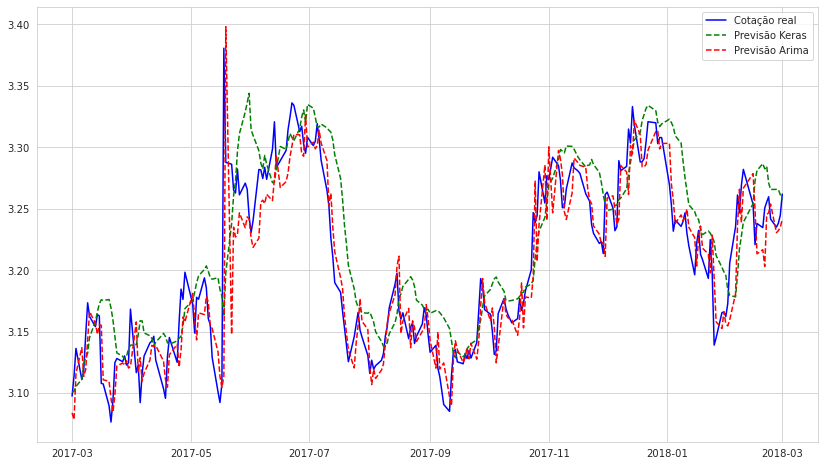
\includegraphics[width=14cm]{figuras/series_previsoes_ano_1}
\caption{Previsões de um ano dos modelos ARIMA, Rede Neural Keras e Média-Móvel $7$ dias das janelas de cotações do Dólar.}
\label{fig:previsoes_ano_1}
\end{figure}

Estão listados na Tabela \ref{tabela:teste_ano_1} os resultados de todos os modelos utilizados, com as métricas de avaliação utilizadas. A partir desses resultados podemos ver que o modelo ARIMA foi o melhor, seguido pelo modelo de Média-Móvel $7$ dias, e em terceiro a Rede Neural Keras, com valores muito próximos entre esses dois últimos.

\begin{table}[]
\begin{center}
\resizebox{\textwidth}{!}{
\begin{tabular}{|c|c|c|c|c|c|}
\hline
\multirow{2}{*}{\textbf{Métrica}} 
& \textbf{Média-Móvel} & \textbf{Média-Móvel} 
& \multirow{2}{*}{\textbf{ARIMA}}
& \textbf{Rede Neural} & \textbf{Rede Neural} \\
& \textbf{(7 dias)} & \textbf{(30 dias)}  
&& \textbf{(Keras)} & \textbf{(Perceptron)} \\
\hline
\hline
\textbf{MAE} & 0.026 & 0.045 & 0.019 & 0.031 & 0.068 \\
\textbf{RMSE} & 0.036 & 0.057 & 0.030 & 0.041 & 0.082 \\
\textbf{Pearson} & 0.857 & 0.615 & 0.906 & 0.850 & 0.518 \\
\hline
\end{tabular}}
\caption{Métricas das previsões para um ano dos modelos das janelas de cotações do Dólar.}\label{tabela:teste_ano_1}
\end{center}
\end{table}

É importante lembrar que a otimização dos modelos ARIMA foi feita separadamente para cada janela de dados de teste, assim como as médias-móveis, por definição, capturam a tendência central de cada janela, enquanto que no caso das Redes Neurais, todo um período fixado do passado é utilizado como treinamento e as previsões foram feitas a partir dos parâmetros ajustados apenas no passado.

Os demais modelos, que não tiveram bons desempenhos, o Perceptron e o modelo de Média-Móvel $30$ dias que troca de lugar com o de $7$ dias que desta vez ficou entre os melhores, estão nos gráficos da Figura \ref{fig:previsoes_ano_2}.

\begin{figure}[htb]
\centering
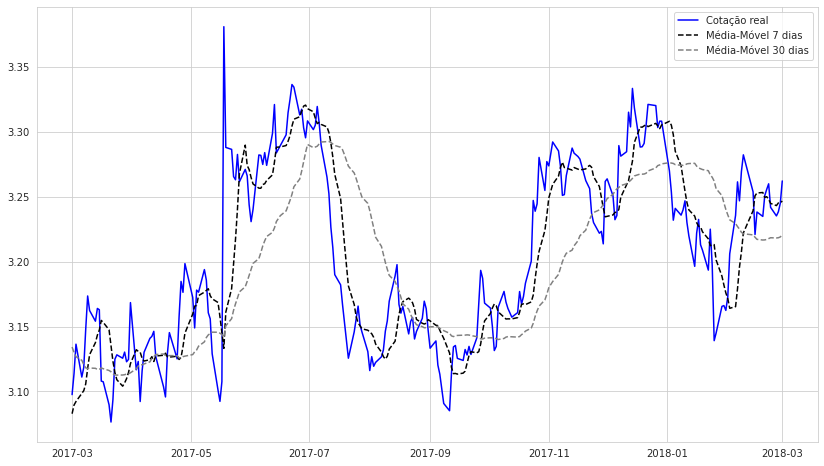
\includegraphics[width=14cm]{figuras/series_previsoes_ano_2}
\caption{Previsões de um ano do modelo de rede Perceptron e de Média-Móvel de $30$ dias das janelas de cotações do Dólar.}
\label{fig:previsoes_ano_2}
\end{figure}

Por fim, é interessante mostrar que no caso do modelo ARIMA, há um intervalo de confiança que é gerado para cada previsão, sendo o padrão do modelo utilizado um nível de confiança de $95\%$, que pode ser visualizado, sombreado ao redor do gráfico das previsões, na Figura \ref{fig:series_arima_ano}.

\begin{figure}[htb]
\centering
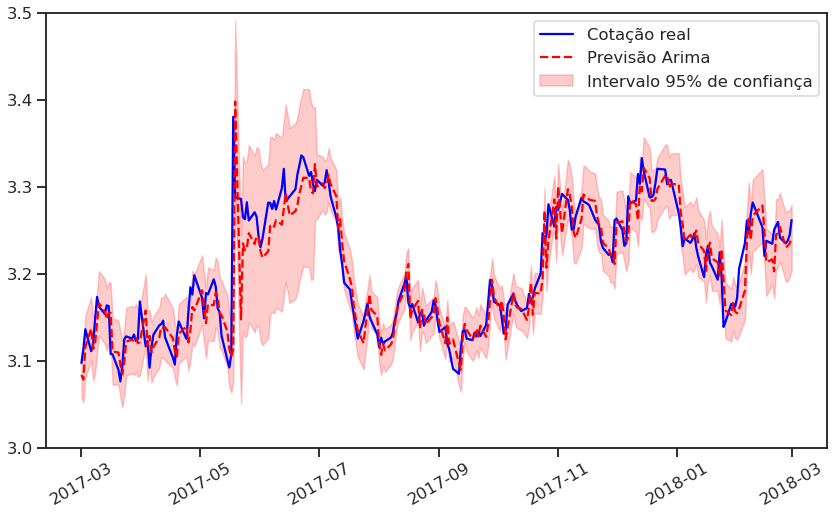
\includegraphics[width=14cm]{figuras/series_arima_ano}
\caption{Previsões do modelo ARIMA com o intervalo de $95\%$ de confiança para cada previsão.}
\label{fig:series_arima_ano}
\end{figure}


\section{Tempos de processamento}

Uma última medida importante a ser comparada, neste tipo de tarefa, diz respeito ao tempo de processamento dos algoritmos de treinamento. Todos os procedimentos foram feitos num ambiente \eng{Jupyter notebook}, que possui comandos muito simples que podem ser utilizados para essa medição\footnote{Foi utilizado o comando $\%\%time$}.

Foi produzida a Tabela \ref{tabela:desempenho} que contém o tempo de processamento do treinamento dos modelos principais aqui comparados, para cada um dos três testes realizados neste capítulo. Nesta tabela estão contabilizados o tempo do \eng{grid search}, no caso do ARIMA, e das épocas de treinamento para os dois modelos de redes neurais.

\begin{table}[]
\begin{center}
\begin{tabular}{|c|c|c|c|}
\hline
\backslashbox{Modelo}{Teste} & \textbf{$7$ dias} & \textbf{$30$ dias} & \textbf{$1$ ano} \\
\hline
\hline
\textbf{Keras} & $< 1$ min & $< 1$ min & $< 1$ min \\
\textbf{Perceptron} & $\sim 2$ min & $\sim 2$ min & $\sim 8$ min \\
\textbf{ARIMA} & $\sim 2$ min & $\sim 10$ min & $\sim 100$ min \\
\hline
\end{tabular}
\caption{Tempo de processamento do treinamento dos modelos de previsão.}\label{tabela:desempenho}
\end{center}
\end{table}